\documentclass[a4paper,11pt]{article}
%
%--------------------   start of the 'preamble'
%
\usepackage{graphicx,amssymb,amstext,amsmath}
\usepackage[usenames]{color}
\usepackage{bm}
\usepackage {hyperref}
\usepackage{caption}
\usepackage{xcolor}
\usepackage[many]{tcolorbox}

\captionsetup[figure]{labelfont=bf,font={small, sf, it}}
\newcommand\etc{\textsl{etc}}
\newcommand\eg{\textsl{eg.}\ }
\newcommand\etal{\textsl{et al.}}
\newcommand\Quote[1]{\lq\textsl{#1}\rq}

\newcommand{\ket}[1]{| #1 \rangle}
\newcommand{\bra}[1]{\langle #1 |}
\newcommand{\braket}[2]{\langle #1 | #2 \rangle}
\newcommand{\proj}[1]{| #1\rangle\!\langle #1 |}
\newcommand{\id}{\mathbbm{1}}
\newcommand{\heff}{\tilde H}
\newcommand{\ueff}{\tilde U}
\newcommand{\nv}{N$-V$}
\newcommand{\nfourteen}{$^{14}$N}
\newcommand{\nfifteen}{$^{15}$N}
\newcommand{\cthirteen}{$^{13}$C}
\newcommand{\ctwelve}{$^{12}$C}
\newcommand {\Fig}[1] {Figure~\ref{#1}}
\newcommand{\dev}[2]{\frac{d #1}{d #2 }}
\newcommand{\secdev}[2]{\frac{d^2 #1}{d #2^2 }}
\newcommand{\ddp}[2]{\frac{\partial #1}{\partial #2 }}
\newcommand{\secpdev}[2]{\frac{\partial^2 #1}{\partial #2^2 }}
\newcommand{\be}{\begin{equation}}
\newcommand{\ee}{\end{equation}}
\newcommand{\ba}{\begin{eqnarray}}
\newcommand{\ea}{\end{eqnarray}}
\def\tr{\mbox{tr}}
\def\la{\mbox{$\langle$}}
\def\ra{\mbox{$\rangle$}}

\renewcommand{\sf}{\sffamily}
\renewcommand{\b}{\bf\sffamily}
\newcommand{\ita}{\it\sffamily}


\newenvironment{exercise}[1]
    {\begin{tcolorbox}[colback=yellow!10!white,
                     colframe=white!20!black,
                     title=#1,  
                     center, 
                     valign=top, 
                     halign=left,
                     before skip=0.8cm, 
                     after skip=1.2cm,
                     center title, 
                     width=12cm]
    }
    {
    \end{tcolorbox}
    }

\setcounter{secnumdepth}{2}
\addtolength{\oddsidemargin}{-.5in}
\addtolength{\evensidemargin}{-.5in}
\addtolength{\textwidth}{1.in}

%---------------------   end of the 'preamble'
%


\begin{document}
\sffamily


\section* {Superconducting quantum devices}

\renewcommand{\labelenumi}{\alph{enumi}.}


\subsection* {Summary}
In this first last week of the course, we will look at a different type of quantum devices, based on superconductivity. Superconductivity is also a purely quantum phenomena, which results in quantum coherence of a macroscopic quantum state, composed by many electrons. Superconducting devices such as SQUIDS are being used as very sensitive magnetometry. One of the main current approaches to quantum computing, pursued for example by Google and IBM, is also based on superconducting quantum devices known as transmon qubits.

Superconductivity is obviously a huge and complex topic in physics, and a deep understanding requires advanced mathematics and quantum mechanics. In just one week, we will take a more phenomenological approach, where we assume that the electrons in a superconductor can be described by a global macroscopic wavefunction $\psi (r, t)$. These notes are heavily based on a beautifully-written masterpiece, the Feynmann Lectures: you can find the source \href{https://www.feynmanlectures.caltech.edu/III_21.html#Ch21-SUM}{here}.


\begin{exercise}{Learning Objectives}
\begin{enumerate}
 \item review the basic concepts of superconductivity (London equations, Meissner effect, etc) through the assumption of a macroscopic quantum model for the superconductor
 \item learn some new phenomena, such as flux quantisation and the Josephson effect
 \item understand the basic working principles of superconducting devices, such as SQUIDs and superconducting single-photon detectors.
\end{enumerate}
\end{exercise}


\subsection* {Resources}
If you want to learn more about this subject, you can consult the following material:
\begin{itemize}
\item {\b book} - C. Kittel, "Introduction to Solid State Physics" (chapter 12)
\item {\b online resource} \href{https://en.wikipedia.org/wiki/Fresnel_equations}{Feynman's Lectures - Chapter 21}
\item {\b scientific paper} \href{https://iopscience.iop.org/article/10.1088/0953-2048/25/6/063001/pdf}{review on superconducting single photon detectors}
\end{itemize}
Keep in mind that notation from different sources might be different than the one used here.

\section {Preliminaries}
This part is taken from the Feynman's lectures, which you can freely access  (\href{https://www.feynmanlectures.caltech.edu/III_21.html#Ch21-SUM}{here}).
\subsection{Probability currents in quantum mechanics}
An important part of the Schrödinger equation for a single particle is the idea that the probability to find the particle at a position is given by the absolute square of the wave function. It is also characteristic of the quantum mechanics that probability is conserved in a local sense. When the probability of finding the electron somewhere decreases, while the probability of the electron being elsewhere increases (keeping the total probability unchanged), something must be going on in between. In other words, the electron has a continuity in the sense that if the probability decreases at one place and builds up at another place, there must be some kind of flow between. If you put a wall, for example, in the way, it will have an influence and the probabilities will not be the same. So the conservation of probability alone is not the complete statement of the conservation law, just as the conservation of energy alone is not as deep and important as the local conservation of energy. If energy is disappearing, there must be a flow of energy to correspond. In the same way, we would like to find a “current” of probability such that if there is any change in the probability density (the probability of being found in a unit volume), it can be considered as coming from an inflow or an outflow due to some current. This current would be a vector which could be interpreted this way—the x-component would be the net probability per second and per unit area that a particle passes in the x-direction across a plane parallel to the yz-plane. Passage toward +x is considered a positive flow, and passage in the opposite direction, a negative flow.

Is there such a current? Well, you know that the probability density $P(r,t)$ is given in terms of the wave function by
\begin{equation}
P(r,t)=\psi^*(r,t)\psi(r,t)    
\end{equation}

I am asking: Is there a current J such that
\begin{equation}
    \ddp{P}{t} = -\nabla \cdot J?
\end{equation}

If we take the time derivative of this equation, we get two terms:
\begin{equation}
\ddp{P}{t}=\psi^*\,\ddp{\psi}{t}+\psi\,\ddp{\psi^*}{t}.
\end{equation}
Now use the Schrödinger equation—Eq. (21.3)—for $\ddp{\psi}{t}$; and take the complex conjugate of it to get $\ddp{\psi^*}{t}$ - each $i$ gets its sign reversed:

\begin{equation}
\begin{aligned}
\ddp{P}{t}&=-\frac{i}{\hbar}\biggl[\psi^*\,\frac{1}{2m}
\biggl(\frac{\hbar}{i}\,\nabla-q\biggr)\cdot
\biggl(\frac{\hbar}{i}\,\nabla-q\biggr)\psi+
q\phi\psi^*\psi\\
&\hphantom{{}={}}-\psi\,\frac{1}{2m}
\biggl(-\frac{\hbar}{i}\,\nabla-q\biggr)\cdot
\biggl(-\frac{\hbar}{i}\,\nabla-q\biggr)\psi^*
-q\phi\psi\psi^*\biggr].
\end{aligned}
\end{equation}

The potential terms and a lot of other stuff cancel out. And it turns out that what is left can indeed be written as a perfect divergence. The whole equation is equivalent to

\begin{equation}
\ddp{P}{t}=-\nabla{\biggl \lbrace
\frac{1}{2m}\,\psi^*
\biggl(\frac{\hbar}{i}\,\nabla-q\biggr)\psi+
\frac{1}{2m}\,\psi
\biggl(-\frac{\hbar}{i}\,\nabla-q\biggr)\psi^*
\biggr \rbrace}.
\end{equation}

It is really not as complicated as it seems. It is a symmetrical combination of $\psi^*$ times a certain operation on $\psi$, plus $\psi$ times the complex conjugate operation on $\psi^*$. It is some quantity plus its own complex conjugate, so the whole thing is real - as it ought to be. The operation can be remembered this way: it is just the momentum operator $P - qA$. We could write the current as:
\begin{equation}
\label{eq:current}
J =\frac{1}{2}\biggl \lbrace
\psi^*\biggl[\frac{\hat{\mathcal{P}}-q \mathbf{A}}{m}\biggr]\psi+
\psi\biggl[\!\frac{\hat{\mathcal{P}}-q \mathbf{A}}{m}\biggr]^*\psi^*
\biggr \rbrace.
\end{equation}

Equation \ref{eq:current} shows that the probability is conserved locally. If a particle disappears from one region it cannot appear in another without something going on in between. Imagine that the first region is surrounded by a closed surface far enough out that there is zero probability to find the electron at the surface. The total probability to find the electron somewhere inside the surface is the volume integral of P. But according to Gauss’s theorem the volume integral of the divergence $J$ is equal to the surface integral of its normal component. If $\psi$ is zero at the surface, Eq. \ref{eq:current} says that $J$ is zero, so the total probability to find the particle inside can’t change. Only if some of the probability approaches the boundary can some of it leak out. We can say that it only gets out by moving through the surface—and that is local conservation.
\begin{comment}
\subsection{(Optional) Some words on momentum}
{\it This part is optional, not compulsory to pass the course}
The equation for the current is rather interesting, and sometimes causes a certain amount of worry. You would think the current would be something like the density of particles times the velocity. The density should be something like $\psi \psi^*$, which is right. And each term in Eq. \ref{eq:current} looks like the typical form for the average-value of the operator

\begin{equation}
\frac{\mathcal{\hat{P}}-qA}{m},
\label{eq:P}
\end{equation}

so maybe we should think of it as the velocity of flow. It looks as though we have two suggestions for relations of velocity to momentum, because we would also think that momentum divided by mass, should be a velocity. The two possibilities differ by the vector potential.

It happens that these two possibilities were also discovered in classical physics, when it was found that momentum could be defined in two ways.7 One of them is called “kinematic momentum,” but for absolute clarity we will call it here the “mv-momentum.” This is the momentum obtained by multiplying mass by velocity. The other is a more mathematical, more abstract momentum, sometimes called the “dynamical momentum,” which I’ll call “p-momentum.” The two possibilities are



It turns out that in quantum mechanics with magnetic fields it is the p-momentum which is connected to the gradient operator $\mathcal{\hat{P}}$, so it follows that Eq. \ref{eq:P} is the operator of a velocity.

I’d like to make a brief digression to show you what this is all about - why there must be something like Eq. (21.15) in the quantum mechanics. The wave function changes with time according to the Schroedinger equation. If I would suddenly change the vector potential, the wave function wouldn’t change at the first instant; only its rate of change changes. Now think of what would happen in the following circumstance. Suppose I have a long solenoid, in which I can produce a flux of magnetic field (B-field). And there is a charged particle sitting nearby. Suppose this flux nearly instantaneously builds up from zero to something. I start with zero vector potential and then I turn on a vector potential. That means that I produce suddenly a circumferential vector potential A. You’ll remember that the line integral of A around a loop is the same as the flux of B through the loop. Now what happens if I suddenly turn on a vector potential? According to the quantum mechanical equation the sudden change of A does not make a sudden change of $\psi$; the wave function is still the same. So the gradient is also unchanged.

But remember what happens electrically when I suddenly turn on a flux. During the short time that the flux is rising, there’s an electric field generated whose line integral is the rate of change of the flux with time:
\begin{equation}
    E = -\ddp{A}{t}
\end{equation}
That electric field is enormous if the flux is changing rapidly, and it gives a force on the particle. The force is the charge times the electric field, and so during the build up of the flux the particle obtains a total impulse (that is, a change in $mv$) equal to $-qA$. In other words, if you suddenly turn on a vector potential at a charge, this charge immediately picks up an $mv$-momentum equal to $-qA$. But there is something that is not changed immediately and that’s the difference between $mv$ and $-qA$. And so the sum $p=mv+qA$ is something which is not changed when you make a sudden change in the vector potential. This quantity $p$ is what we have called the $p$-momentum and is of importance in classical mechanics in the theory of dynamics, but it also has a direct significance in quantum mechanics. It depends on the character of the wave function, and it is the one to be identified with the operator
\begin{equation*}
\mathcal{P}=\frac{\hbar}{i}\,\nabla.
\end{equation*}
\end{comment}

\section {The macroscopic quantum model of superconductivity}
\subsection {The assumptions}
You have already seen the phenomenology of superconductivity in the "Condensed Matter" course last semester, with an introduction to the most exciting effects.

Here we discuss a simple model of superconductivity known as "macroscopic quantum model" for superconductivity because it is based on the assumption that there exists a macroscopic coherent wave function
\begin{equation}
    \psi (r;t) = \sqrt{\rho(r; t)} e^{i\theta(r; t)},
\end{equation}
which describes the behavior of the whole ensemble of superconducting electrons. In this hypethesis, all the electrons in the superconductor can be described by a single wavefunction, with a well defined phase. This is in contrast to what happens in a standard metal, where the phases associated with the different electrons are all different from each other.

This hypothesis can be justified by the microscopic theory of superconductivity (BCS-theory). The BCS theory, developed by Bardeen, Cooper and Schrieffer, is based on the idea that in superconducting metals there is an attractive force between electrons near the Fermi level. At temperatures below the critical temperature $T_c$ this
attractive force creates a new quantum state differing from the Fermi sea of a normal metal. Roughly we can say that a small portion of the electrons close to the Fermi level are bound into {\bf Cooper pairs}.
\newline In the simplest case, the internal motion of the pairs has no orbital angular momentum (symmetric state) and consequently Pauli’s principle requires that the two spins must be in a singlet (antisymmetric) spin state. In contrast to binding of two atoms to a molecule, the orbital state of the pair has a much larger radius typically between 10 nm and 1 mm so that the individual pairs overlap strongly in space and consequently the binding turns cooperative. In particular, the binding energy of any pair depends on how many other pairs have condensed and, furthermore, the center of mass motion of the pairs is so strongly correlated that each pair resides in the same state with the same center of mass motion.
\newline It turns out that this attractive interaction between electrons, that leads to the formation of Cooper pairs, is mediated by the interaction of each electron with the phonons in the crystal lattice.



Let us now go back to the wavefunction $\psi (r;t) = \sqrt{\rho(r; t)} e^{i\theta(r; t)}$ describing the superconductor. It is clear what the density $\rho$ means - but what is the physical significance of the phase $\theta(r; t)$?

If we substitute $\psi (r)$ into Eq. \ref{eq:current}, and express the current density in terms of these new variables $\rho$ and $\theta$, we get:

\begin{equation}
\label{eq:SC_J}
J=\frac{\hbar}{m}\biggl(
\nabla \theta - \frac{q}{\hbar}\,\mathbf{A}\biggr)\rho.
\end{equation}

Since both the current density and the charge density have a direct physical meaning for the superconducting electron gas, both $\rho$ and $\theta$ are real physical quantities. The absolute phase is not observable, but if the gradient of the phase is known everywhere, the phase is known except for a constant. You can define the phase at one point, and then the phase everywhere is determined.

\subsection {London Equations and the Meissner effect}
If we take the curl in both side of Eq. \ref{eq:SC_J}, we get:
\begin{equation}
    \nabla \times \mathbf{J} = \frac{q \rho}{m} \mathbf{B}
\end{equation}
where we have used that the curl of a gradient of a scalar is zero. This is one of the {\bf London equations} that you have already encountered in "Condensed Matter".

From this, one can derive the Meissner effect. From Maxwell's equation we know that:
\begin{equation}
    \mathbf{\nabla} \times \mathbf{B} = \mu_0 \mathbf{J}
\end{equation}
If we take the curl of both sides, we get:
\begin{equation}
    \mathbf{\nabla} \times \mathbf{\nabla} \times \mathbf{B} = \mu_0 \mathbf{\nabla} \times \mathbf{J}
\end{equation}
From vector calculus we know that $\nabla \times \nabla \times B = -\nabla^2 B$, and therefore:
\begin{equation}
    -\mathbf{\nabla}^2 B = \mu_0 \mathbf{\nabla} \times \mathbf{J}
\end{equation}
If we now use London's equation, we get to:
\begin{equation}
    \mathbf{\nabla}^2 \mathbf{B} = \frac{1}{\lambda_L^2} \mathbf{B}
\end{equation}
where $\lambda_L = \sqrt{\frac{m}{\mu_0 q \rho}}$.

This equation tells us that a magnetic field decays exponentially as:
\begin{equation}
    B(x) = B(0)e^{-x/\lambda_L}
\end{equation}
and cannot penetrate into a superconductor ({\bf Meissner effect}).

\subsection {Flux quantisation}
Let us now consider a ring of superconducting material. Inside the body of the ring the current density is zero, therefore Eq. \ref{eq:SC_J} tells us that:
\begin{equation}
    \mathbf{\nabla} \theta = \frac{q}{\hbar} \mathbf{A}
\end{equation}
Over a closed path $C$ through the interior of the superconducting ring:
\begin {equation}
\hbar \oint_C \mathbf{\nabla} \theta \cdot d\mathbf{s} = q \oint_C \mathbf{A} \cdot d\mathbf{s}
\end{equation}
On the right side, we can use Stokes theorem and transform a line integral on $\mathbf{A}$ to an integral of $\mathbf{\nabla} \times \mathbf{A} = \mathbf{B}$ across a surface delimited by $C$:
\begin{equation}
    \oint_C \mathbf{A} \cdot d\mathbf{s} = \oint_C (\mathbf{\nabla} \times \mathbf{A}) \cdot d\mathbf\sigma = \oint_C \mathbf{B} \cdot d\sigma = \Phi
\end{equation}
This is the magnetic flux $\Phi$ across the loop.

On the left side, we are taking an integral over the gradient of the phase $\theta$. For a path from point $1$ to point $2$, this would just be the difference between the values of $\theta$ at points $1$ and $2$:
\begin{equation}
    \hbar \oint_C \mathbf{\nabla} \theta \cdot d\mathbf{s} = \hbar \left( \theta_2 - \theta_1 \right)
\end{equation}
For a closed path, where the start point and end point coincide, one could naively assume that this difference is zero. However, $\theta$ is a phase, so it could still differ by multiples of $2\pi$ for the expression to be valid.

Putting left and right side together we get:
\begin{equation}
    \Phi = \frac{2\pi \hbar}{q} n
\end{equation}
i.e. the magnetic flux is quantised in multiples of $2 \pi \hbar/q$!

In 1961 such a quantized flux was looked for and found by Deaver and Fairbank at Stanford University and at about the same time by Doll and Nabauer in Germany.

In the experiment of Deaver and Fairbank, a tiny cylinder of superconductor was made by electroplating a thin layer of tin on a one-centimeter length of copper wire. The tin becomes superconducting below $3.8$K while the copper remains a normal metal. The wire was put in a small controlled magnetic field, and the temperature reduced until the tin became superconducting. Then the external source of field was removed. You would expect this to generate a current by Lenz’s law so that the flux inside would not change. The little cylinder should now have magnetic moment proportional to the flux inside. The magnetic moment was measured by jiggling the wire up and down (like the needle on a sewing machine, but at the rate of 100 cycles per second) inside a pair of little coils at the ends of the tin cylinder. The induced voltage in the coils was then a measure of the magnetic moment.

When the experiment was done by Deaver and Fairbank, they found that the flux was quantized, but that the basic unit was only one-half as large as London had predicted. Doll and Nabauer got the same result. At first this was quite mysterious, but we now understand why it should be so. According to the Bardeen, Cooper, and Schrieffer theory of superconductivity, the charge $q$ which appears in the equation is not the electron charge, but the charge of a pair of electrons and so is equal to $2e$. The basic flux unit is therefore:
\begin{equation}
    \Phi_0 = \frac{\pi \hbar}{2e}
\end{equation}

\section {Josephson junctions}
{\it This section is based on Kittel.}

We have already discussed the phenomenon of quantum tunneling, a quantum effect that enables electrons to pass through very thin barriers. This is, for example, the case of thin ($1-2$nm) insulating layers separating two metals. For normal metals, the tunneling current depends linearly on the applied voltage.

In this section, we will examine structures consisting of two superconductors separated by a thin insulating barrier, known as {\bf weak link}. In this case, the tunneling of Cooper pairs results in quite some distinctive effects.

Let's label $\phi_1$ ($\phi_2$) the macroscopic quantum wavefunction of the Cooper pairs on the left (right) of the junction. We will assume for simplicity that the two superconductors are identical, and we will only decribe one dimension ($x$).

The time-dependent Schoedinger equation 
%\begin{equation}
\begin{align}
i\hbar\,\ddp{\psi_1}{t}&=U_1\psi_1+K\psi_2,\\
i\hbar\,\ddp{\psi_2}{t}&=U_2\psi_2+K\psi_1.
\end{align}
%\end{equation}

The constant $K$ is a characteristic of the junction. If $K$ were zero, these two equations would just describe the lowest energy state — with energy $U$ — of each superconductor. But there is coupling between the two sides by the amplitude $K$ that there may be leakage from one side to the other. (It is just the “flip-flop” amplitude of a two-state system.) If the two sides are identical, $U_1$ would equal $U_2$ and I could just subtract them off. But now suppose that we connect the two superconducting regions to the two terminals of a battery so that there is a potential difference $V$ across the junction. Then $U_1 - U_2=qV$. I can, for convenience, define the zero of energy to be halfway between, then the two equations are:
\begin{equation}
\begin{aligned}
i\hbar\,\ddp{\psi_1}{t}&=+\frac{qV}{2}\,\psi_1+K\psi_2,\\
i\hbar\,\ddp{\psi_2}{t}&=-\frac{qV}{2}\,\psi_2+K\psi_1.
\end{aligned}
\label{eq:josephson_system}
\end{equation}

\subsection{DC Josephson effect}
Let us first consider the case where no voltage is applied ($V=0$), so that the Eq \ref{eq:josephson_system} above reduce to:
\begin{equation}
\begin{aligned}
i\hbar\,\ddp{\psi_1}{t}&=+K\psi_2,\\
i\hbar\,\ddp{\psi_2}{t}&=+K\psi_1.
\end{aligned}
\end{equation}
If we know use $\psi_i = \sqrt{\rho} e^{i \theta_i}$, we get:
\begin{equation}
\begin{aligned}
\ddp{\psi_1}{t} = \frac{1}{2}\rho_1^{-1/2} e^{i\theta_1} \ddp{\rho_1}{t} + i\psi_1 \ddp{\theta_1}{t} = -K \psi_2\\ 
\ddp{\psi_2}{t} = \frac{1}{2}\rho_2^{-1/2} e^{i\theta_2} \ddp{\rho_2}{t} + i\psi_2 \ddp{\theta_2}{t} = -K \psi_1
\end{aligned}
\end{equation}
If we multiply the first equation on the left by $\rho_1^{1/2} e^{i\theta_1}$ and the second by $\rho_2^{1/2} e^{i\theta_2}$, renaming $\delta = \theta_2 - \theta_1$ we get:
\begin{equation}
\begin{aligned}
\frac{1}{2} \ddp{\rho_1}{t} + i\psi_1 \ddp{\theta_1}{t} = -i K (\rho_1 \rho_2)^{1/2} e^{i\delta}\\ 
\frac{1}{2} \ddp{\rho_2}{t} + i\psi_2 \ddp{\theta_2}{t} = -i K (\rho_1 \rho_2)^{1/2} e^{-i\delta}
\end{aligned}
\end{equation}

If we consider separately the real and imaginary parts for each of the equations, we get the following four equations:
\begin{equation}
\begin{aligned}
\ddp{\rho_1}{t} &= 2K (\rho_1 \rho_2)^{1/2} \sin{\delta}\\
\ddp{\theta_1}{t} &= - K \left(\frac{\rho_2}{\rho_1}\right)^{1/2} \cos{\delta}\\ 
\ddp{\rho_2}{t} &= -2K (\rho_1 \rho_2)^{1/2} \sin{\delta}\\
\ddp{\theta_2}{t} &= - K \left (\frac{\rho_1}{\rho_2} \right)^{1/2} \cos{\delta}
\end{aligned}
\end{equation}
For identical superconductors we can take the density of Cooper pairs to be the same on both sides of the junction ($\rho_1 \sim \rho_2$, leading to:
\begin{equation}
    \ddp{\theta_1}{t} = \ddp{\theta_1}{t} \longrightarrow \delta = \mbox{const} 
\end{equation}
Given that the current is proportional to $\ddp{\rho}{t}$, we get:
\begin{equation}
    J  = J_0 \sin{\delta} = J_0 \sin \left( \theta_2 - \theta_1 \right)
\end{equation}
This equation tells us that, even when no voltage is applied across the junction, a current still flows, proportional to the sine of the phase difference between the wavefunctions of the Cooper pairs on the left and on the right of the junction. This is known as {\bf DC Josephson effect}.

\subsection{AC Josephson effect}
Let us now go back to Eq. \ref{eq:josephson_system} and consider the case of a voltage $V$ applied to the junction. An electron pair experiences a potential energy difference $qV$ on passing across the junction where $q=-2e$. 
If we proceed exactly as above, we end up with the four equations:
\begin{equation}
\begin{aligned}
\ddp{\rho_1}{t} &= 2K (\rho_1 \rho_2)^{1/2} \sin{\delta}\\
\ddp{\theta_1}{t} &= \left( \frac{eV}{\hbar}\right)- K \left(\frac{\rho_2}{\rho_1}\right)^{1/2} \cos{\delta}\\ 
\ddp{\rho_2}{t} &= -2K (\rho_1 \rho_2)^{1/2} \sin{\delta}\\
\ddp{\theta_2}{t} &= -\left( \frac{eV}{\hbar}\right) - K \left (\frac{\rho_1}{\rho_2} \right)^{1/2} \cos{\delta}
\end{aligned}
\end{equation}
Now the phase different is not constant anymore, but we have:
\begin{equation}
    \delta(t) = \delta(0) - \frac{2eV}{\hbar}
\end{equation}
Therefore, the current oscillates in time with a frequency $\omega = 2eV/\hbar$:
\begin{equation}
    J = J_0 \sin \left[ \delta(0) - \frac{2eV}{\hbar}t \right]
\end{equation}
At non-zero bias, the weak link therefore behaves as a voltage-controlled oscillator. A DC voltage of $1 \mu$V applied to the device, for example, produces an oscillating current at a frequency of $483.6$ MHz. This has been used, among other things, to obtain a very precise measurement of $e/\hbar$. Since this relationship of voltage to frequency involves only fundamental constants and since frequency can be measured with extreme accuracy, the Josephson junction has become the standard voltage measurement. 

\section {Superconducting Quantum Interference Devices (SQUIDs)}
Let us consider now two Josephson junctions in parallel, with no voltage applied. The ends, P and Q, are connected to our electrical instruments which measure any current flow. The external current, $J_{tot}$, will be the sum of the currents through the two junctions. Let $J_a$ and $J_b$ be the currents through the two junctions, and let their phases be $\delta_a$ and $\delta_b$. The phase difference of the wave functions between P and Q must be the same whether you go on one route or the other. Along the route through junction “a”, the phase difference between P and Q is $\delta_a$, which (as we have seen when describing flux quantisation) is related to the flux $\Phi$ as $\delta_a = \delta_0 - \frac{e}{\hbar c} \Phi $. A similar expression ($\delta_a = \delta_0 + \frac{e}{\hbar c} \Phi $) is valid for $\delta_b$, such that the phase difference between the two paths is given by:
\begin{equation}
    \delta_b- \delta_a = \frac{2e}{\hbar c} \Phi 
\end{equation}
The total current is the sum of $J_a$ and $J_b$:
\begin{equation}
    J_{tot} = J_0 \lbrace \sin \left( \delta_0 + \frac{e}{\hbar c} \Phi \right) + J_0 \lbrace \sin \left( \delta_0 -  \frac{e}{\hbar c} \Phi \right)  \rbrace = 2 \left( J_0 \sin \delta_0 \right) \cos \left( \frac{e}{\hbar c} \Phi \right)
\end{equation}

\begin{figure}[h]
\centering
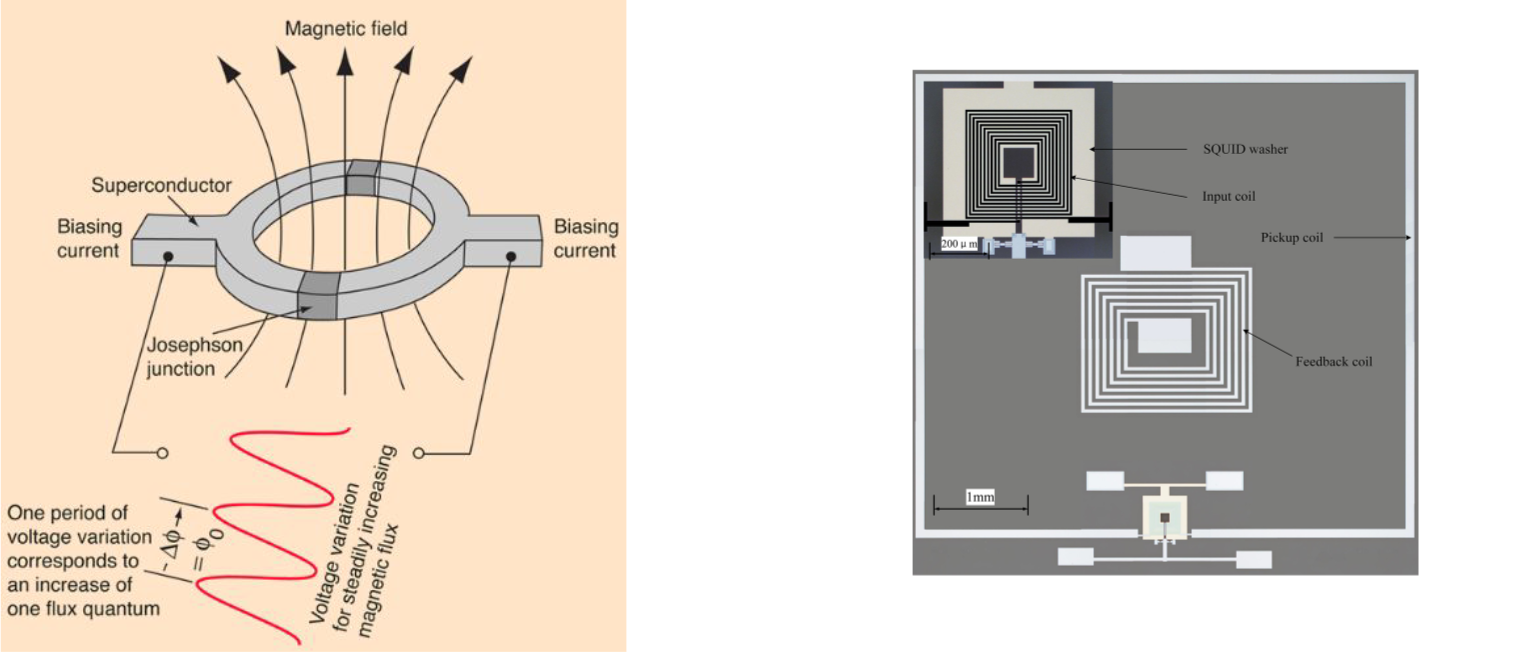
\includegraphics[width = 1\textwidth]{figures/SQUID.png}
\caption{On the left, working principles of a SQUID (from \href{http://hyperphysics.phy-astr.gsu.edu/hbase/Solids/Squid.html}{"hyperphysics"}). On the right, optical microscope image of a complete SQUID device.}
\label{fig:SQUID}
\end{figure}

The current is therefore periodic as a function of the flux $\Phi$, and thereby as a function of the magnetic field through the SQUID loop. A SQUID, therefore, can operate as a magnetic field sensor. The evaluation of the voltage-flux curve allows to resolve magnetic field changes down to $\sim 10^{-18}$T. This makes SQUIDs successful devices in many research areas, for example, to detect very weak magnetic fields associated to heart or brain currents. One important thing to consider is that a SQUID detects a magnetic flux, therefore the signal is larger for a larger loop area (at the expense of spatial resolution). Scanning-SQUID geomtetries, with a small SQUID fabricated on a scanning nano-tip, have also been demonstrated.

{\bf Fabrication} Low-$T_c$ SQUIDs are almost exclusively fabricated from niobium (Nb) thin-films. Niobium has a transition temperature of about $9.25$ K, well above the boiling temperature of liquid helium, and is mechanically very stable. High-quality films can  be  fabricated  by  electron-beam  evaporation  or  by  sputtering.  Tunnel  junctions are  patterned  from Nb/AlO/Nb trilayers in which the AlO barrier is formed by oxidization of a few nanometers of Al. The films are patterned with standard optical photolithography with linewidths down to a few micrometers. The photoresist stencil is transferred to the underlying film by “lift-off” or dry etching techniques. Niobium films can be selectively etched using reactive ion etching. For magnetometers and gradiometers, one often forms a hybrid with a wire-wound pickup loop bonded to the thin-film input coil.

\begin{figure}[h]
\centering
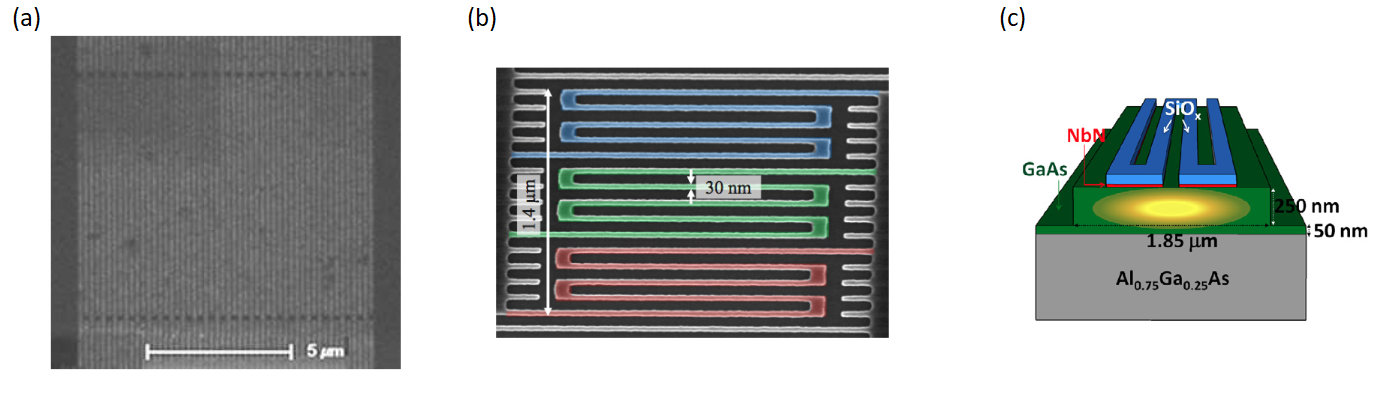
\includegraphics[width = 1\textwidth]{figures/SSPD_devices.png}
\caption{Example of SSPD devices. {\bf(a)} SEM photo of a Nb meander SSPD device covering a $10 \mu$m by $10 \mu$m area. {\bf(b)}) Ultra-thin nanowires (30 nm wide) are connected in parallel to improve the sensitivity of the SSPD.{bf (c)} f) A SSPD device fabricated directly on top of an optical waveguide structure, to improve the optical coupling efficiency. (Figure from \cite{natarajan_superconducting_2012})}
\label{fig:SSPD_device}
\end{figure}



\section {Superconducting Single Photon Detectors}
In quantum photonics application, the detection of single photons is a crucial task. This is typically performed with avalanche photodiodes (APDs), i.e. photodiodes biased close to the break-down point, where even the small energy associated with one single photon is sufficient to trigger an avalanche of photo-electrons through carrier multiplication in a heavily-doped region. While single-photon APDs have been very successful, they also have some drawbacks, in particular:
\begin{enumerate}
    \item they provide high detection efficiency and relatively low noise in the visible, but in the near-infrared (important, for example, for telecommunications in the $1550$ nm band) they suffer from reduced efficiency and a very strong background noise. The background noise consisting of "dark count" events not triggered by the detection of a photon but by thermal excitation of carriers (facilitated by the smaller band-gap of the semiconductors used for detection in the infrared)
    \item in terms of speed, it is hard to reduce jitter below a few hundred picoseconds
\end{enumerate}

\begin{figure}[h]
\centering
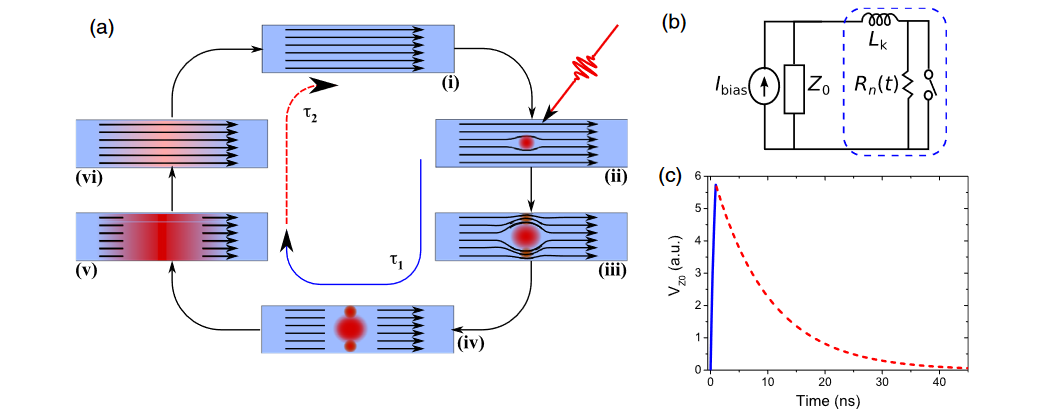
\includegraphics[width = 1\textwidth]{figures/SSPD_operation.png}
\caption{{\bf (a)} Physics principles for SSPD operation, as described in the text. {\bf (b)}  A simple electrical equivalent circuit of a SSPD. $L_k$ is the kinetic inductance of the superconducting nanowire and $R_n$ is the hotspot resistance of the SSPD. The SSPD is current biased at $I_{bias}$. Opening and closing the switch simulates the absorption of a photon. An output pulse is measured across the load resistor $Z_0$. {\bf (c)} A simulation of the output voltage pulse of the SSPD (approximating the pulse shape typically observed on an oscilloscope after amplification). Values of $L_k=500$ nH and $R_n=500 \Omega$ have been used. (Figure from \cite{natarajan_superconducting_2012})}
\label{fig:SSPD_oper}
\end{figure}


In the last decade or so, several research groups have developed a novel concept for photon detection, based on superconductivity. Superconducting single-photon detectors offer several advantages, and are commercially available by several vendors worldwide.

Superconducting nanowire single-photon detector (SSPD/SNSPD) consiste of a thin nanowire of superconducting material (NbN) arranged in a meander geometry. The basic device operation can be described as follows : 
\begin{enumerate}
    \item The superconducting nanowire maintained well below the critical temperature is direct current (DC) biased just below the critical current.
    \item A photon  absorbed by the nanowire has enough energy to disrupt hundreds of Cooper pairs in a superconductor, breaking the superconductivity in a small "hotspot" (which becomes normal).
    \item The supercurrent is forced to flow along the periphery of the hotspot. Since the NbN nanowires are narrow, the local current density around the hotspot increases, exceeding the superconducting critical current density. 
    \item This in turn leads to the formation of a resistive barrier across the width of the nanowire
    \item Joule heating (via the DC bias) aids the growth of resistive region along the axis of the nanowire until the current flow is blocked and the bias current is shunted by the external circuit.
    \item This allows the resistive region to subside and the wire becomes fully superconducting again. The bias current through the nanowire returns to the original value
\end{enumerate}

\begin{figure}[h]
\centering
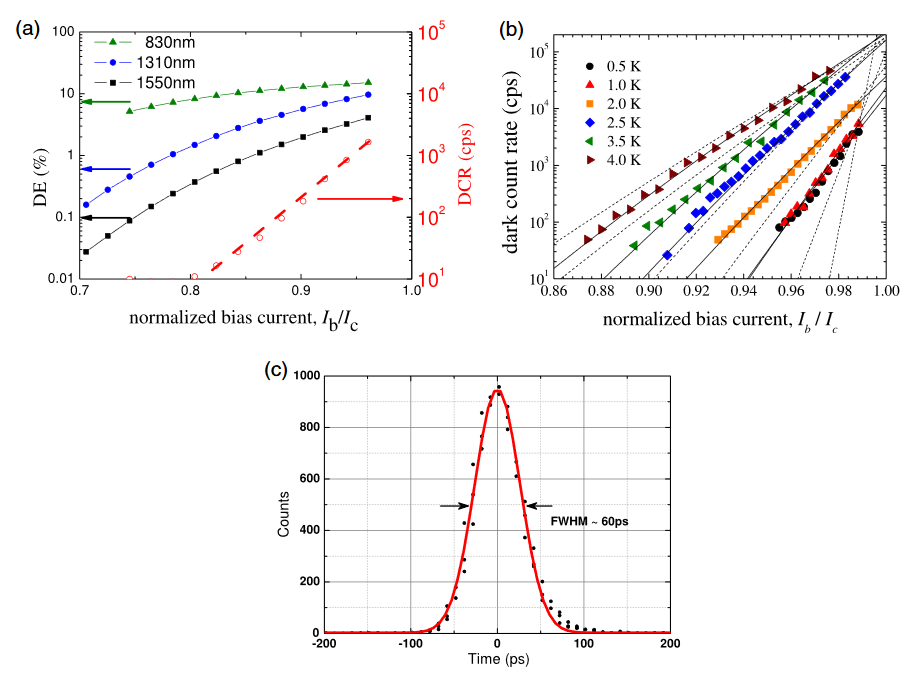
\includegraphics[width = 1\textwidth]{figures/SSPD_performance.png}
\caption{{bf(a)} Detector efficiency (left y-axis) as a function of the bias current, for different wavelengths. {bf(b)} Dark counts as a function of the bias current at different operating temperatures. Clearly, the lower the operating temperature, the lower the dark count rate (for the same bias current). {bf(c)} Temporal resolution of a typical SSPD detector, on the order of $\sim 50$ps. (Figure from \cite{natarajan_superconducting_2012})}
\label{fig:SSPD_perf}
\end{figure}


SSPD performance is illustrated in Fig. \ref{fig:SSPD_perf}. The detection efficiency increases for high bias current, as the dark count rate. The count rate, however, decreases when lowering the operation temperature. Therefore, one should operate at the lowest possible temperature, while finding a bias current that gives the right trade-off between signa and noise.

SSPDs are nowadays widely used in research labs (there are several sytems operating at Heriot-Watt) and in industrial settings (for example for semiconductor optical testing).

\section {Superconducting Qubits}
we have discussed last week Kane's proposal for a quantum computer based on spins in silicon. An alternative proposal, currently pursued by big industrial players such as Google and IBM, is based on superconducting qubits. We will here just provide a qualitative explanation of the working principles behind this approach.

\begin{figure}[h]
\centering
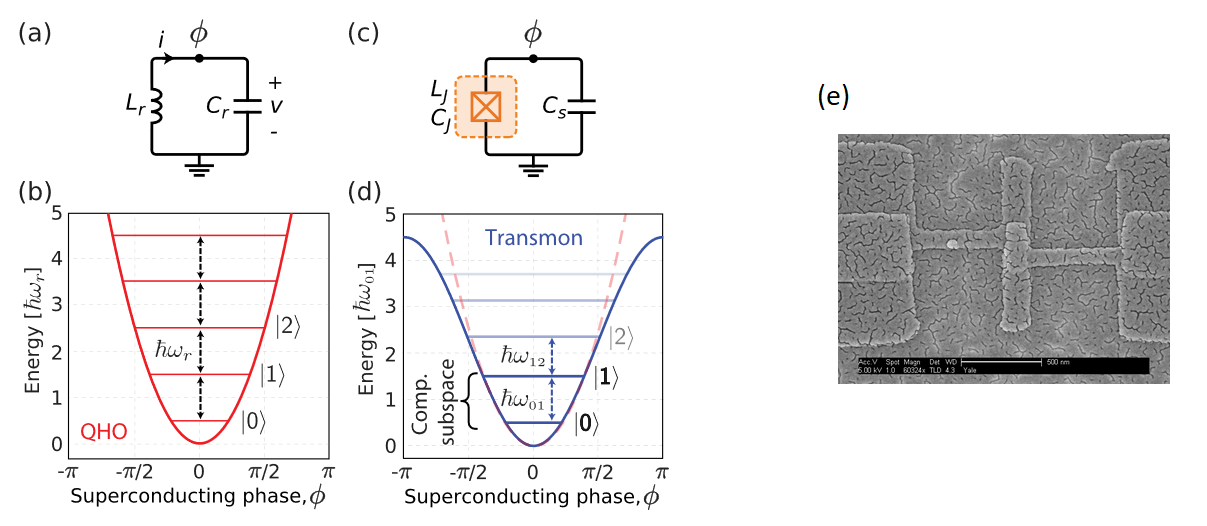
\includegraphics[width = 1\textwidth]{figures/transmon.png}
\caption{On the left, an $LC$ circuit behaves as a perfect harmonic oscillator, with energy levels equally-spaces such that no selective address is possible (given that all transitions connecting nearby levels have the same frequency). A modified circuit with a Josephson junction operating as a nonlinear inductor, on the other hand, introduces a small anharmonicity, which removes the degeneracy in the excitation frequencies, enabling the isolation of a two-level system. On the right, SEM photo of a transmon. The Josephon junction consists of the two overlapping stripes in the centre, which are separated by a very thin oxide layer. }
\label{fig:transmon}
\end{figure}

You have seen the concept of quantum harmonic oscillator several times during your studies, typically associated with a mass-spring model of oscillating phenomena such as photons or phonons. Another phenomenon that can be described by a harmonic oscillator is an $LC$ electrical circuit. A quantum harmonic oscillator has energy levels equally spaced by energy $h \omega$: of course, this is problematic to implement a qubit because we have an infinite number of states, all driven by the same frequency $\omega$.
\newline To be able to isolate two states to work as a qubit, one can introduce a non-linearity, modifying the parabolic potential. This can be done with a Josephson junction, which behaves as a non-linear inductor, transforming the $LC$ circuit into a two-level system. Such structure is the basis of what is called a {\bf transmon}, the basic building block at the core of current state-of-the-art quantum computing research.

Such a two-level system can be controlled with microwave radiation at the proper frequency, exactly as the spin qubits we have seen previously. Additionally, the transmon is typically coupled to a microwave cavity to enhance interaction with single microwave photons. The cavity-transmon system operates in the {\bf strong coupling} regime of cavity-QED, which will be familiar to those of you who followed B21NT "Nanophotonics" last semester. Concepts from strong-coupling cavity-QED (which, for this case, it is also labeled {\bf circuit QED}) enable single-shot qubit readout.

Quantum computing schemes based on transmon qubits are currently among the leading candidates, with Google recently reporting the demonstration of a quantum algorithm implemented on a record number of $53$ qubits \cite{arute_quantum_2019}. The main issue with this architecture is, however, the requirement to operate at mK temperatures.

\bibliography{nanophysics_bib}
\bibliographystyle{ieeetr}
\end{document}
